\section{Modo Depuración}

La información respecto al movimiento de nuestros agentes la podemos consultar en el inspector en la parte derecha de unity siempre y cuando no ejecutemos el juego en pantalla completa. Para intentar hacer que algunos valores se consulten de forma más intuitiva se ha hecho uso de Gizmos y también de imágenes auxiliares.

Empezando por los Gizmos, estos son una clase especial de Unity que nos permite que sea activada y desactivada durante la ejecución a través del inspector como se ve en la figura \ref{fig:giz} y estos serán visibles en la escena.

\begin{figure}[H]
    \centering
    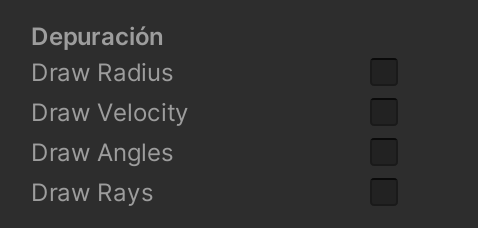
\includegraphics[scale=0.5]{images/Gizmos.png}
    \caption{Gizmos disponibles}
    \label{fig:giz}
\end{figure}

Para que una clase pueda `depurar' sus atributos será necesario que esta tenga un método llamado \texttt{OnDrawGizmos}. Veamos por ejemplo el de la clase \texttt{Agent} que muestra los atributos de la figura anterior. 

\lstinputlisting[linerange=190-230, firstnumber=190]{\ScriptsPath/Steering/NPC/Agent.cs}

En este bloque de código vemos como se comprueban si están activados cada una de las casillas. Cada subbloque estable el color y la forma en la que se verán los distintos gizmos. Por ejemplo, en el subbloque de \texttt{drawRadius}, se puede ver como se dibujan dos círculos de distintos colores alrededor del agente, representando cada uno de ellos los radios del agente.

El otro elemento introducido a modo de depuración del comportamiento de los agentes, ha sido el de poder conocer el estado en el que está cada uno mediante el icono de estado que aparece a la izquierda del personaje. La implementación de este mecanismo ya se explicó en la sección \ref{sec:interfaz}, \textit{Interfaz gráfica y Jugabilidad}.